\chapter{引言}


\section{研究背景}

随着软件与硬件技术的不断发展进步,摄像头已经成为人们日常生活中必不可少的互联网设备。摄像头的发展更加趋向于模块化,功能化,小型化,应用场景也更加广泛。在智能手机上,前置和后置摄像头成为必备设备;在安防监控领域,摄像头正在被大量布置;在自动驾驶以及其他自动控制领域,摄像头正在替代人眼成为信息输入的主要来源。同时得益于处理器计算能力地不断增强,在摄像头模块中也集成了更多的实用功能,摄像头不再仅仅作为图像采集设备。例如,利用摄像头实现人脸识别功能,替代密码输入或者进行人员搜索;利用摄像头实现运动物体检测功能,在监控过程中替代人工监视;利用摄像头实现图像处理分析,实时生成周围环境信息。摄像头越来越强大的功能给人们的日常生活提供了巨大帮助。

但是,对于单一摄像头,其成像大小、拍摄速率等方面仍存在一定的限制。因此将多个摄像头整合到一起,组成多摄像头系统,成为摄像头发展的一个重要方向。这样既可以利用不同性能参数的摄像头弥补各自的不足之处,也可以成倍扩展摄像头性能。同时,多摄像头系统可以由多个参数指标一般,较为便宜普通的摄像头组成,通过系统优化使其实现更高的性能。

例如,Stanford大学计算机图形学实验室利用100个低成本的CMOS摄像头组成了一个大规模阵列,配合相应的编码器、FPGA、处理器和控制总线等设备,通过调整各摄像头的排列顺序和拍摄角度,实现了高像素、高帧率、多光场摄影等功能 \cite{1}。当将各摄像头紧密排列,通过同步使其在同一时间拍摄,将拍摄到的所有图像进行拼接,可以得到一幅高像素的图像,即利用低像素多摄像头系统进行高像素拍摄。当控制各摄像头在不同时间拍摄相同图像,将各帧图像按时间顺序排列,可以突破各个摄像头拍摄帧率的限制,在每秒内得到更多图像,即利用低帧率摄像头实现高速摄影。当各摄像头之间存在一定距离,该系统即可实现多焦点拍摄,得到光场图像数据。

\begin{figure}[h] 
  \centering
  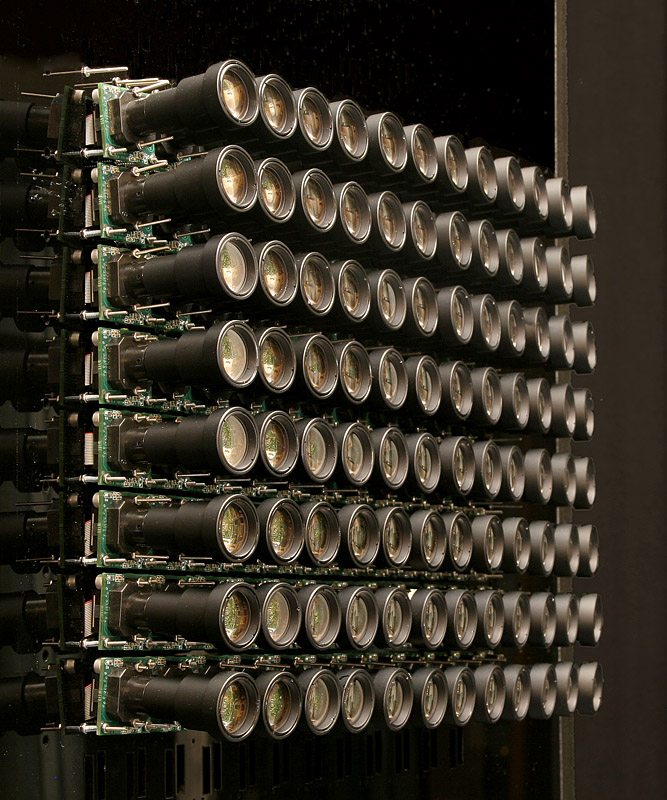
\includegraphics[height=6cm, width=7cm]{Stanford}
  \caption{Stanford大学多摄像头阵列}
  \label{Stanford}
\end{figure}


同样,在智能手机领域,越来越多的智能手机配备了双目摄像头系统。例如Apple公司的iPhone 7手机和华为公司的P9手机,均配备双目摄像头,这样可以有效优化拍摄图像的亮度、对比度和清晰度等,以获得更好的拍摄效果。诺基亚公司曾发布过一款智能手机,使用的是一颗摄像头阵列,包含4 × 4共16颗子镜头,为了提高图片的色彩纯净度,每个子镜头仅捕捉红、绿、蓝三种颜色当中的一种,由处理器对所有子镜头拍摄到的图像进行叠加处理,这样还能够更好地抑制噪点。该手机使用的摄像头阵列还能够实现多点变焦功能,即在拍摄时,各个子镜头选取不同的焦点,并将所有拍摄数据保存,这样可以实现一次拍摄,得到不同焦点的图像。在拍摄后期,就可以根据需要选取合适的焦点调整图片效果。

\begin{figure}[h]
  \centering%
  \subcaptionbox{包含16颗子镜头的阵列摄像头模块}
    {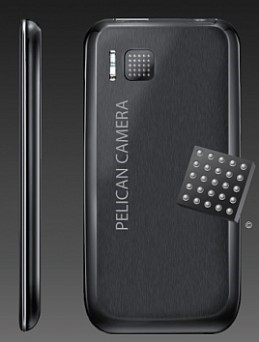
\includegraphics[height=6cm]{nokia1}}
  \subcaptionbox{选取不同焦点,在后期对图片进行变焦处理}%[5cm]
    {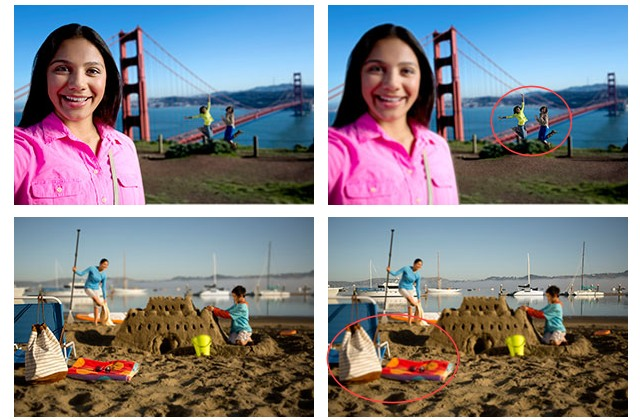
\includegraphics[height=6cm]{nokia2}}
  \caption{诺基亚阵列摄像头手机}
  \label{nokia}
\end{figure}

在无人驾驶领域,特斯拉第二代自动驾驶技术的摄像头系统包括了三个前置摄像头,即一个主摄像头负责采集主要道路信息,一个配备广角镜头的副摄像头检测更多车道,一个副摄像头检测前方车辆;在四旋翼飞行器领域,大疆公司最新的精灵4 Pro飞行共器配备了7个摄像头,安装在机身周围的摄像头可以实现躲避障碍物、追踪拍摄对象等功能,安装在机身下方的摄像头可以实现精确定位、悬停等功能,同时高分辨率、高帧率的主摄像头可以实现4K高清视频的拍摄;在VR、3D视频拍摄领域,需要多摄像头实现多角度全景拍摄,或模拟人眼拍摄立体视觉效果。多摄像头系统在越来越多的领域得到了广泛应用,发挥了越来越重要的作用,也越来越受到人们的重视。

\begin{figure}[h]
  \centering%
  \subcaptionbox{特斯拉自动驾驶技术}
    {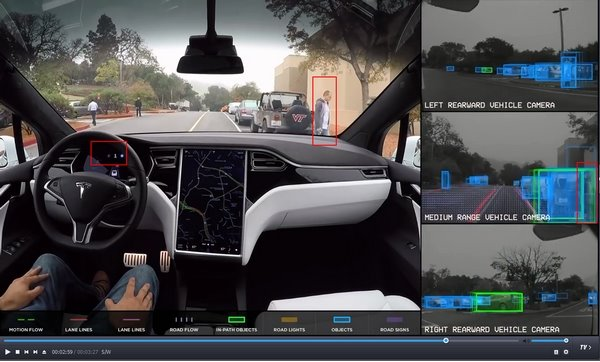
\includegraphics[height=4cm, width=4.7cm]{tesla}}
  \subcaptionbox{大疆四旋翼飞行器}%[5cm]
    {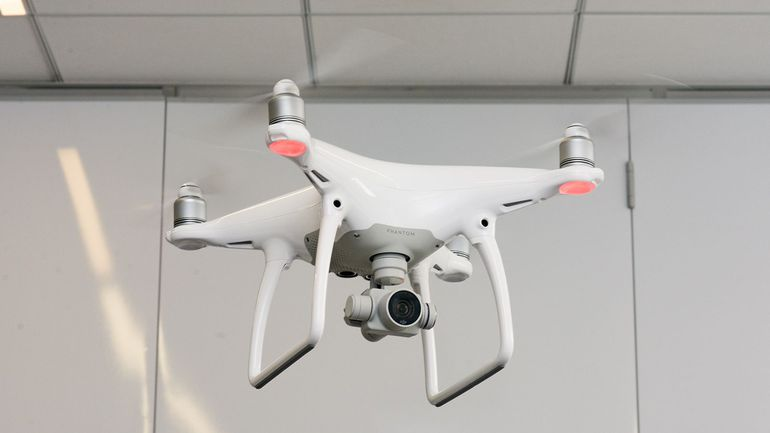
\includegraphics[height=4cm, width=4.7cm]{dji}}
  \subcaptionbox{诺基亚全景VR相机}%[5cm]
    {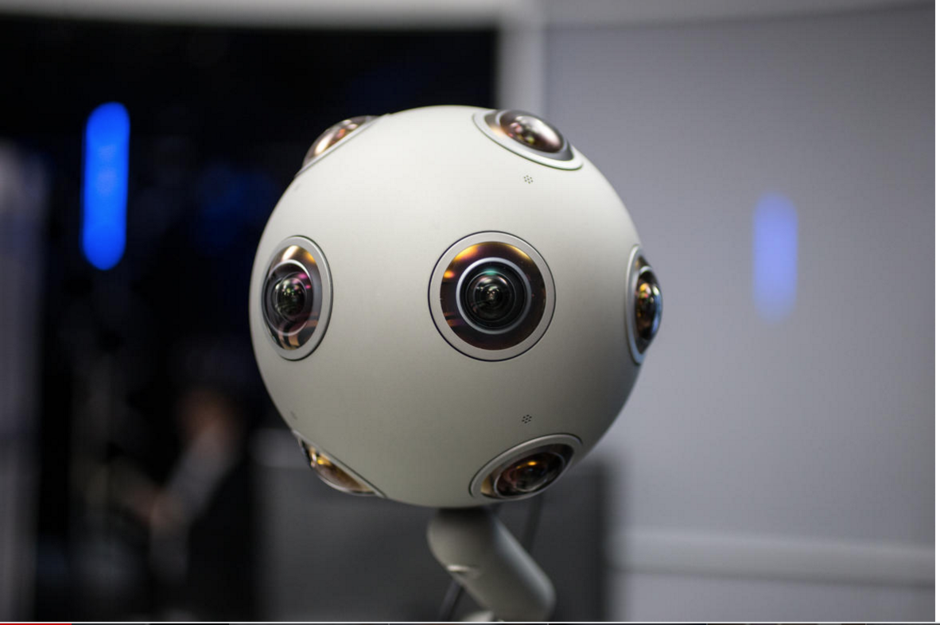
\includegraphics[height=4cm, width=4.7cm]{ozo}}
  \caption{多摄像头系统的应用场景}
  \label{camera}
\end{figure}


目前关于多摄像头系统的研究主要集中在软件应用和硬件优化两个方面。其中,软件应用主要是利用现有的成熟系统实现或优化特定功能。例如对多摄像头图像进行拼接校准,利用多摄像头系统进行目标跟踪识别,利用多摄像头系统进行全景拍摄三维重建等。此类应用大多在现有的多摄像头系统的基础上采集数据,或者直接利用拍摄好的视频文件进行研究,因此对于多摄像头系统的性能参数并没有较严格的要求。而关于硬件优化方面的研究,主要集中于如何搭建多摄像头系统,包括摄像头控制,数据传输,算法优化,视角调整等。此方面的研究资料较少,主要是因为对于硬件系统的研究需要耗费大量的人力物力,且属于基础研究,能够取得的突破性成果较少。

对于多摄像头系统来说,为了实现其特定的功能,需要控制系统内的各个摄像头在同一时刻拍摄或按照特定的时间间隔拍摄。如果为了将各个摄像头拍摄到的图像进行拼接,以得到更大分辨率的图像,就需要各个摄像头精确地在同一时刻进行拍摄,这样才能捕捉到拍摄对象在该时刻的状态,如果拍摄时间存在间隔,则拍摄对象的状态发生变化,就无法进行准确的拼接。如果为了将各个摄像头拍摄到的图像按时间顺序穿插排列,以得到更高的拍摄速率,就需要各个摄像头的拍摄时间存在一定的时间差。例如,对于一个双摄像头系统来说,各个摄像头的拍摄速率为25帧每秒(Frames Per Second,FPS),即各个摄像头拍摄的每两帧图像之间的时间间隔为40ms,如果控制两个摄像头的拍摄时间间隔为20ms,则第一个摄像头拍摄的第一帧图像与第二个摄像头拍摄的第一帧图像之间相差20ms,第二个摄像头的第一帧图像与第一个摄像头的第二帧图像相差20ms。将所有拍摄图像按时间顺序交错排列,即可得到每帧图像之间相差20ms的视频,其拍摄速率即为50FPS,该系统利用两个摄像头实现了帧率的提升。

而部分研究工作对各个摄像头之间的时间间隔并没有提出明确的要求,是由于时间差对其研究结果造成的影响较小。例如在进行图像拼接时,如果各个摄像头拍摄静态对象,那么在较短的时间段内,拍摄对象发生的变化不大。而如果对较快的运动对象进行拍摄时,在一定的时间段内,拍摄对象就会发生较大变化从而影响拼接结果。如图~\ref{subfig1} 所示,待拼接的对象为静态的建筑物,两张图片的拍摄时间即使存在一定的差别仍然不影响拍摄结果。而如图~\ref{subfig2} 所示,当拍摄对象为移动的人时,如果拍摄时间不同,则拼接后的图像中同一个人会出现两次,且动作不同 \cite{2}。

\begin{figure}[h]
  \centering%
  \subcaptionbox{静态拍摄对象的图像拼接\\. \label{subfig1}}
    {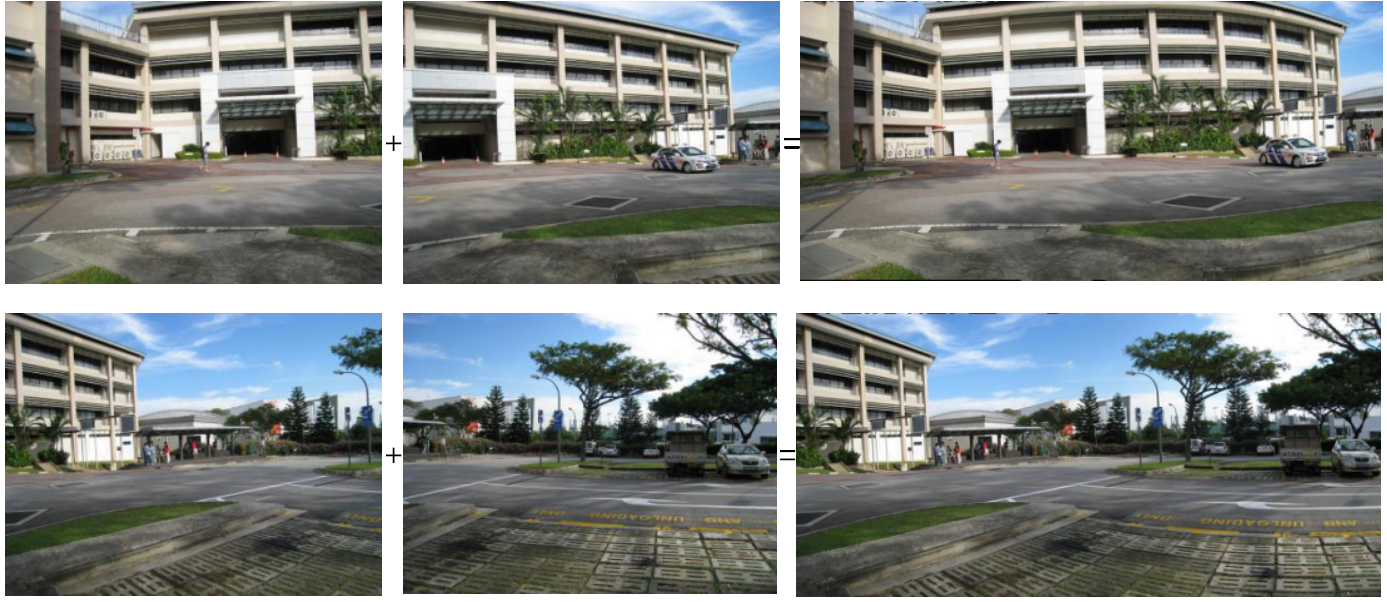
\includegraphics[height=6.5cm]{sitch1}}
    \hspace{4em}%
  \subcaptionbox{动态拍摄对象的图像拼接\label{subfig2}}
      {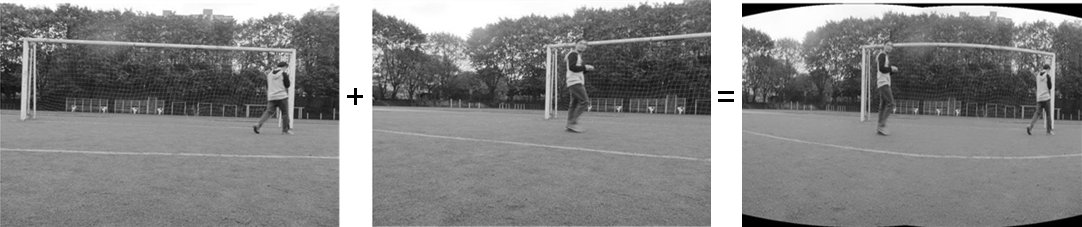
\includegraphics[height=3cm]{sitch2}}
  \caption{拍摄时间存在间隔时进行图像拼接的结果}
  \label{sitch}
\end{figure}

因此,在多摄像头系统的搭建过程当中,一个重要的问题在于如何实现系统内各个摄像头之间的时间同步。目前主要的同步方法有硬件同步和软件同步两种。硬件同步指的是利用硬件设备将控制系统与各个摄像头相连,通过控制信号控制摄像头的拍摄时间。如图~\ref{multi}所示CODEX多摄像头控制器,即可实现对多个摄像头的控制及数据传输功能\footnote{https://www.provideocoalition.com/codex-multi-camera-recorder/}。同样还可以利用外部信号,如闪光灯、声音等控制各个摄像头。如图~\ref{camera}所示的由单反相机组成的阵列即可以利用闪光灯作为触发信号,实现“子弹时间”的拍摄。利用软件对多摄像头系统进行同步,主要是指由服务器控制各个摄像头,根据采集到的图像数据分析拍摄时间,从而判定系统内的同步情况,最后根据算法对摄像头进行调整。

\begin{figure}[h]
  \centering%
  \subcaptionbox{CODEX多摄像头控制器 \label{multi}}
    {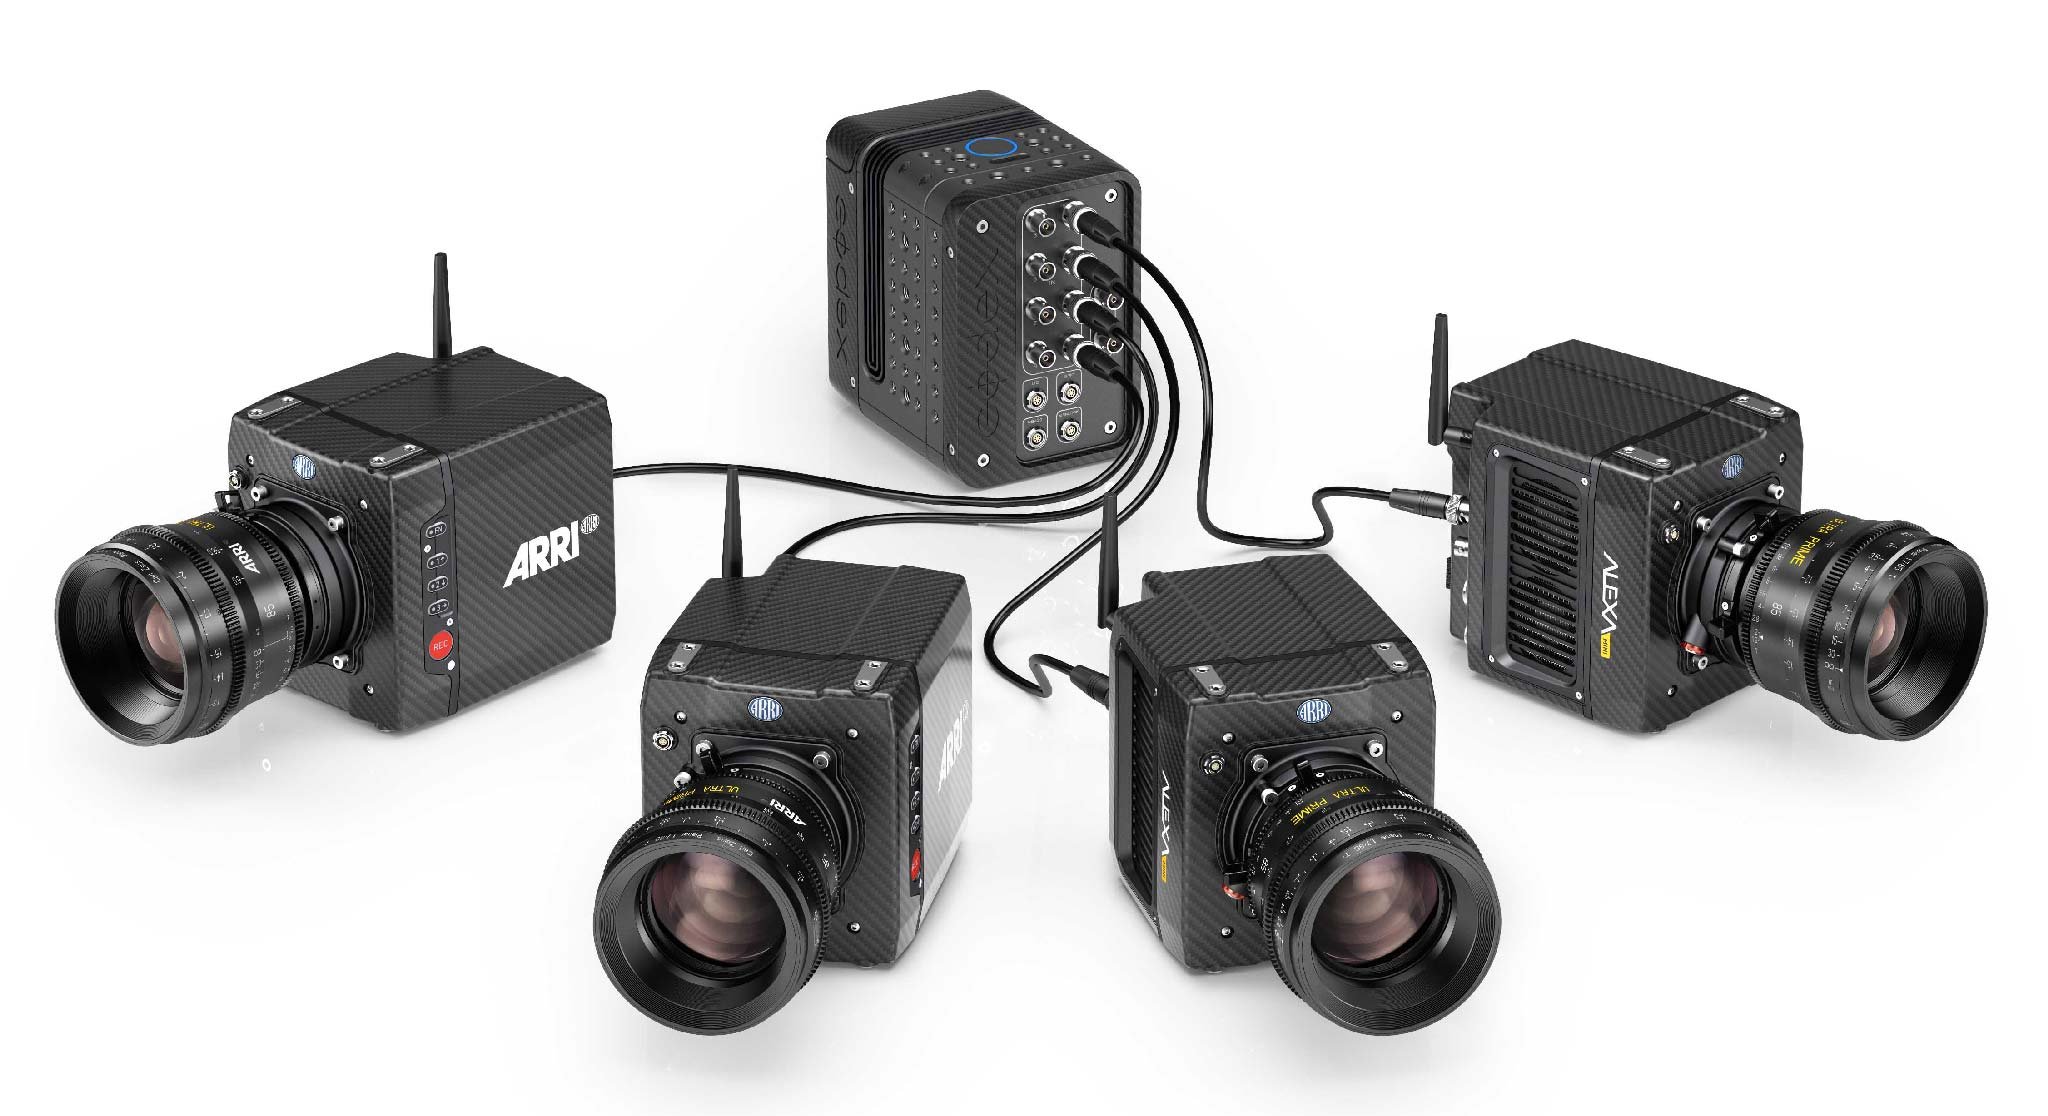
\includegraphics[height=4cm, width=6.cm]{multi}}
    \hspace{4em}%
  \subcaptionbox{闪光灯触发多摄像头阵列\label{camera}}
      {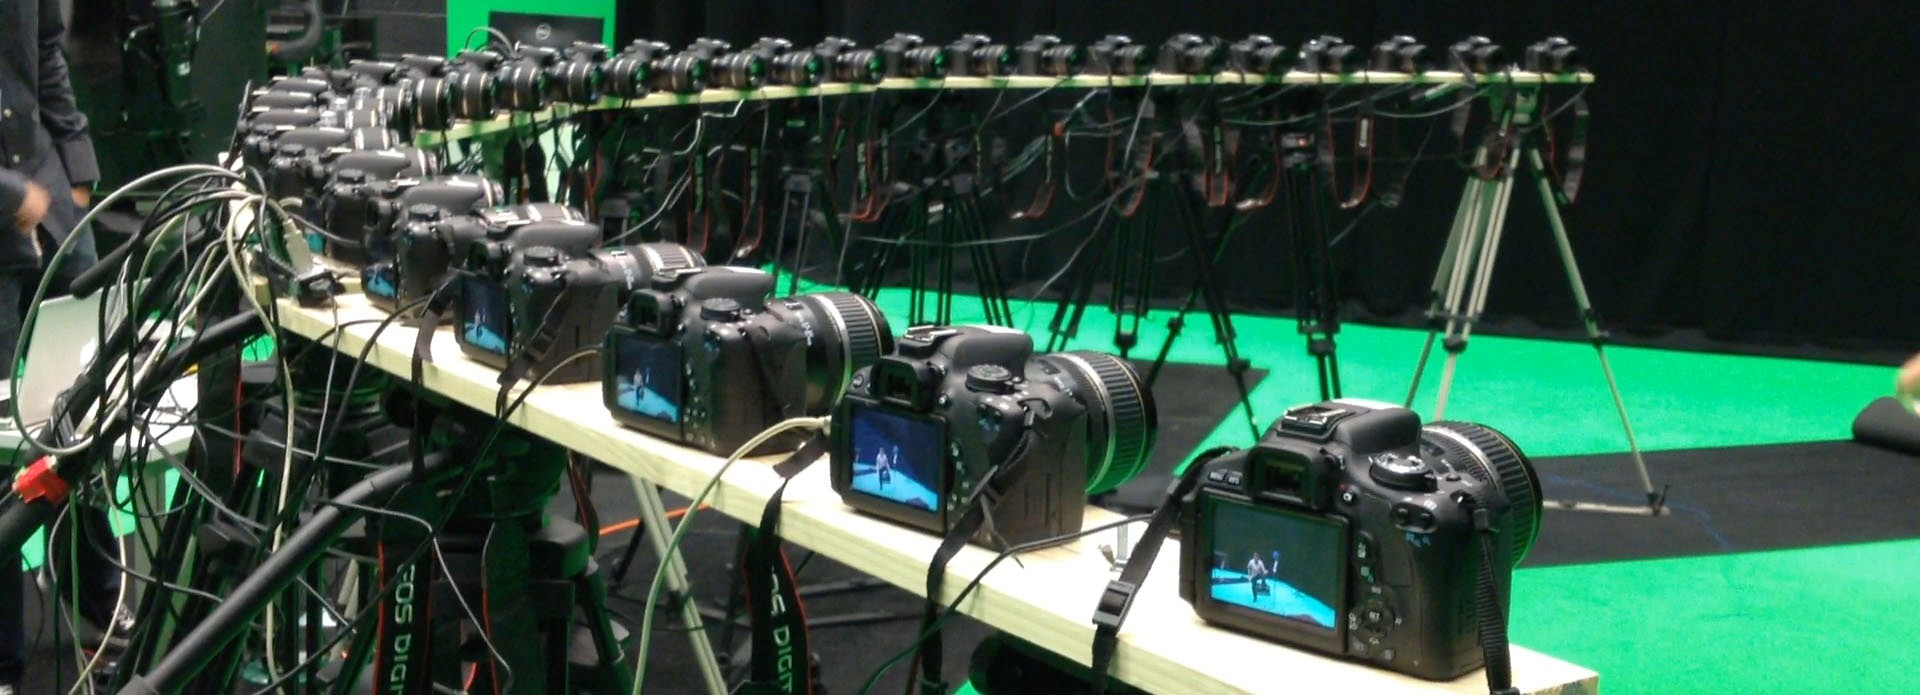
\includegraphics[height=4cm, width=6.7cm]{camera}}
  \caption{利用硬件进行多摄像头同步}
\end{figure}

在对多摄像头系统进行同步的过程中,大部分方法是根据摄像头或者控制系统产生的时间戳来判定摄像头拍摄时间的,即这些方法认为时间戳生成的时间与摄像头的曝光时间严格一一对应,这种方法在对同步精度要求不高的情况下是可以被认为是正确的。但是在实际操作过程当中,多摄像头系统内系统响应、信号传输、软件运行都会耗费长短不等且随机分布的时间,因此从控制单元想摄像头发送拍摄指令到生成时间戳,再到摄像头的感光器件开启曝光,这之间会存在随机变化的时间间隔,也就导致系统生成的时间戳无法精确表示摄像头拍摄时间,各个摄像头之间可能会与控制要求存在误差。

因此,对于需要精确同步的多摄像头系统来说,还需要有时间戳以外的方法来精确表示摄像头的拍摄时间,即如何检测摄像头的拍摄时间也是多摄像头系统实现过程当中的一个重要问题。目前应用较多的方法是利用灯光信号作为时钟信号,被摄像头拍摄后根据拍摄图像识别拍摄时刻的信号信息,从而确定摄像头的拍摄时刻。

\section{主要研究内容和挑战}


\section{本文的主要贡献}








































